%30/01 - Raúl Guantes
\chapter{Conceptos básicos}
\section{La importancia de cuantificar y estimar las escalas en biología}
La biología de sistemas es un campo que busca entender los sistemas biológicos a través de la cuantificación y la modelización matemática. Los modelos matemáticos son simplificaciones de sistemas biológicos complejos, y aunque no son perfectos (ya que no pueden capturar toda la información), son útiles para entender y predecir comportamientos biológicos. Como dijo el estadístico George Box: "Todos los modelos son erróneos, pero algunos son útiles".

Una herramienta clave en este campo es BioNumbers, una base de datos que recopila información cuantitativa en biología. Esta información es esencial para interpretar resultados experimentales y diseñar nuevos experimentos. Por ejemplo, al realizar experimentos, es fundamental calcular la media y la desviación estándar de los resultados para estimar el error. El error se redondea a una cifra significativa, y la medida se expresa con la misma precisión que el error.

\subsection{Estimación de la expresión de proteínas en \textit{E. coli}}
Supongamos que encontramos una proteína en un cultivo celular de \textit{E. coli} con una concentración de 1 picoMolar (pM) por célula. ¿Es esta expresión significativa? Para responder, necesitamos calcular el número de moléculas de la proteína por célula, lo que depende del volumen celular.

\paragraph{Datos} Las bacterias tienen forma cilíndrica con una longitud de 2 micras y un diámetro de 1 micra. La concentración de la proteína: $C = 1 pM = 10^{-12}M$.

\paragraph{Cálculos}
\begin{enumerate}
\item Volumen de la célula
$$V = \pi r^2 h \rightarrow \pi (0,5 \mu m)^2 2 \approx 1,5 \mu m^3 = 1,5 \cdot 10^{-15} l = 1,5 fl$$
\item Número de moléculas de proteína por célula
$$C = \frac{N_p}{V \cdot N_{av}} \rightarrow N_p = C \cdot V \cdot N_{av}$$
$$N_p = C \cdot V \cdot N_{av} = 10^{-12}M \cdot 1,5 \cdot 10^{-15}l \cdot 6 \cdot 10^{23} \approx 10^{-3} molecules$$
Esto significa que hay aproximadamente 1 molécula de proteína por cada 1.000 células.
\end{enumerate}

De esta forma, podemos decir que como regla general, una concentración de 1 nanomolar (nM) en \textit{E. coli} corresponde aproximadamente a 1 molécula por célula, dado que el volumen de una célula de \textit{E. coli} es del orden de 1 fl.

\subsection{Variabilidad en la cuantificación de proteínas}
En \textit{E. coli}, la cantidad de proteínas se ha cuantificado utilizando dos técnicas principales: espectrometría de masas y microscopía de fluorescencia. Estas técnicas arrojan resultados diferentes:
\begin{itemize}
\item En espectrometría de masas, el número promedio de una proteína cualquiera en \textit{E. coli} es de 1.000-2.000 moléculas.
\item En microscopía de fluorescencia, este número es de alrededor de 50 moléculas.
\end{itemize}

\begin{figure}[h]
\centering
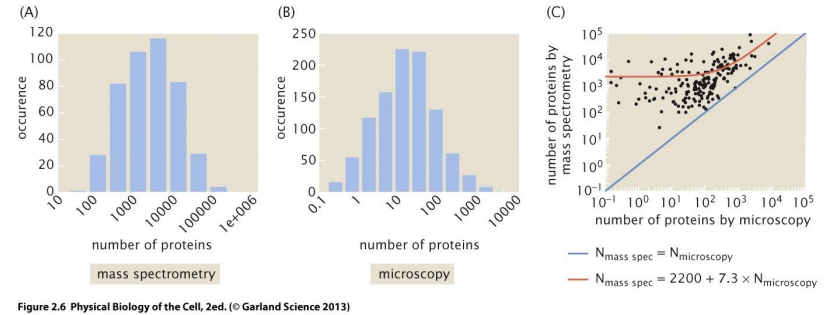
\includegraphics[width = 0.9\textwidth]{figs/mol-census.png}
\end{figure}

Para \textbf{proteínas muy abundantes}, ambas técnicas muestran una buena correlación.
Para \textbf{proteínas poco abundantes}, la correlación se pierde debido a la variabilidad intrínseca en la expresión génica. Esto no es un artefacto experimental, sino una consecuencia de la estocasticidad en los procesos biológicos (limitación física). Cuando el número de copias de una proteína es bajo, la probabilidad de que ocurran reacciones bioquímicas al azar es menor. Esto genera una gran variabilidad en la cantidad de proteínas entre células genéticamente idénticas. En cambio, cuando el número de copias es alto, las reacciones ocurren con mayor frecuencia, reduciendo la variabilidad.

\subsection{Consecuencias numéricas en biología}
La expresión génica es un proceso altamente estocástico debido al bajo número de copias de muchas moléculas involucradas (ADN, factores de transcripción, ARN polimerasa, etc.). Esto tiene varias implicaciones:
\begin{itemize}
\item \textbf{Variabilidad celular:} Incluso en poblaciones de células clonales en el mismo ambiente, la expresión de proteínas varía significativamente. Por ejemplo, las huellas dactilares de dos gemelos son diferentes debido a esta variabilidad.
\item \textbf{Estocasticidad como mecanismo evolutivo:} La aleatoriedad en la expresión génica puede ser aprovechada para generar diversidad. Por ejemplo, en \textit{Bacillus subtilis}, algunas células entran en estado de esporulación en ausencia de nutrientes, mientras que otras continúan dividiéndose.
\end{itemize}

\subsection{Ejemplo: distancia media entre proteínas en una célula de \textit{E. coli}}
La distancia entre proteínas en una célula es inversamente proporcional a la concentración de proteínas (a mayor concentración de proteínas, menos distancia entre ellas). Matemáticamente, siendo c la concentración de proteínas:
$$c = \frac{1}{V_b} = \frac{1}{d^3} \rightarrow d \approx \frac{1}{c^{\frac{1}{3}}}$$

Los cálculos serían los siguientes:
\begin{enumerate}
\item Concentración total de proteínas en \textit{E. coli}:
$$c_{\text{total protein}} = \frac{N^T_p}{V_{E.coli}}$$
\begin{itemize}
\item Peso de \textit{E. coli}: 1 pg. De ahí, el 70\% es agua y el 30\% es masa seca. Las proteínas equivalen al 50\% de la masa seca. Masa total de proteínas en \textit{E. coli}: $0,15 pg = 15 \cdot 10^{-14} g$
\item Sabemos que una proteína tiene de media 300 aminoácidos, y que cada aminoácido tiene una masa media de 100 Dalton. Por tanto, una proteína tiene de media  $3 \cdot 10^4$ Dalton. Un Dalton son $1,7 \cdot 10^{-24}$ gramos. Así:
$$3\cdot 10^4 \cdot 1,7 \cdot 10^{-24} \approx 5 \cdot 10^{-20}$$. 

Masa promedio de una proteína: $5 \cdot 10^{-20} g$

\item Número total de proteínas:
$$N^T_p = \frac{\text{masa total de prot en E. coli}}{\text{masa promedio de 1 proteina}} \rightarrow \frac{15 \cdot 10^{-14}}{5 \cdot 10^{-20}} = 3 \cdot 10^6$$
\item Concentración:
$$c_{\text{total protein}} = \frac{3 \cdot 10^6}{10^9} = 3 \cdot 10^{-3} mol/cel$$
\end{itemize}
\item Distancia media entre proteínas:
$$d = \frac{1}{(3 \cdot 10^{-3})^{\frac{1}{3}}} \approx 7nm$$
\end{enumerate}

El radio típico de una proteína en \textit{E. coli} es de 2-5 nm. Una distancia media de 7 nm indica que las proteínas están muy cerca unas de otras, un fenómeno conocido como "\textbf{molecular crowding}".
Este hacinamiento molecular tiene consecuencias físicas: muchas reacciones bioquímicas están limitadas por la \textbf{difusión lenta} de las moléculas. Por ello, las células han desarrollado estructuras como los microtúbulos para facilitar el transporte y la movilidad, y las constantes de reacción medidas \textit{in vitro} no son iguales a las medidas \textit{in vivo}

\section{Dinámicas en biología}
Todos los sistemas biológicos cambian y evolucionan en el tiempo con una gran diversidad en cuanto a las escalas temporales.
Hay muchos ejemplos en Biología en los que un comportamiento transitorio es importante. Las células perciben señales que pueden codificar información en amplitud, duración y frecuencia.

Los sistemas dinámicos, es decir, sistemas que cambian con el tiempo, se describen con ecuaciones diferenciales, ya que las ecuaciones diferenciales simbolizan la dinámica o velocidad de cambio de las variables que importan en base a otras. Siendo p la cantidad de proteína:
$$\frac{dP}{dt}$$
Si la derivada es negativa, significa que a medida que aumenta el tiempo, la proteína disminuye. Si por el contrario es positiva, entonces la proteína aumenta su expresión en el tiempo. Si la derivada es mucho mayor que 1, aumenta rápido, mientras que si es menor que 1 (pero valor positivo), aumenta despacio. La velocidad de cambio va a ser una función de todas las variables de las que dependa la cantidad de p.
$$\frac{dP}{dt} = f(p, ARN, TF,) \rightarrow f(u, t; \mu)$$
Siendo u las variables dinámicas y $\mu$ los parámetros. u(t) indica las trayectorias o soluciones, por lo que es importante especificar las condiciones iniciales.
Si todas las variables dinámicas aparecen con el exponente 1 como máximo, el sistema es lineal; de lo contrario, se trata de un sistema no lineal.

Las ecuaciones diferenciales ordinarias representan sistemas homogéneros que cambian de forma continua en el tiempo (determinístico). No obstante, generalmente la biología no es así; no hay sistemas totalmente predecibles por fluctuaciones o eventos probabilísticos, y no tienen por qué ser homogéneos. 

En el artículo se ha estudiado el proceso de apoptosis de células tumorales tras dar una droga. Las proteínas se han marcado fluorescentemente, y se puede ver cómo cambian las distintas proteínas tras la adminsitración de la droga. Esto se puede simular de forma precisa, pero estas simulaciones se corresponden a experimentos de los que se obtiene una media poblacional. Las proteínas individuales tienen fluctuaciones en el tiempo. Todas las fluctuaciones están promedidadas, por lo que el modelo de ecuaciones diferenciales determinista simula el promedio de las células. En los experimentos se mide la fluorescencia total en la célula, no su localización subcelular.

Hay otros sistemas en los que las coordenadas espaciales se deben tener en cuenta, como puede ser durante el desarrollo. Cuando se mide el proceso del desarrollo, las células deben mantener constancia de la posición espacial en la que se encuentra. Esto se debe a que las células anteriores se diferencian de forma distinta a las células posteriores. Los genes se expresan en oleadas. En estos casos, se utilizan las ecuaciones diferenciales parciales, teniendo en cuenta el tiempo y las coordenadas espaciales para las variables dinámicas. 

\section{Procesos dinámicos simples celulares: crecimiento celular, dilución proteica y degradación}
El crecimiento celular es constante en cuanto al tiempo.
Siendo N(t) el número de células en un tiempo dado, ¿cuántas células se obtienen al cabo de un tiempo determinado? La variable N cambia a lo largo del tiempo, por lo que hay que utilizar una ecuación diferencial que da la velocidad de cambio de N con el tiempo según la tasa de crecimiento r: 
$$\frac{dN}{dt} = r N \rightarrow r = \frac{1}{T_{div}}$$
Se trata de un sistema lineal con una sola variable. El siguiente paso es la separación de variables para posteriormente derivar. 
$$\frac{dN}{N} = r \cdot dt \rightarrow \int \frac{dN}{N} = \int r \cdot dt \rightarrow \int \frac{dN}{N} = r \cdot \int dt \rightarrow ln N = r t$$
Añadiendo la constante de integración:
$$e^{ln N(t)} = rt + c \rightarrow N(t) = c_0 \cdot e^{rt}$$
Para determinar $c_0$, es necesario especificar condiciones iniciales. Por tanto, hay que establecer que en el momento en el que se inicia el experimento (N(0)), se parte de x células.
$$N(0) = c_0 \cdot e^{r\cdot 0} = c_0$$
Así:
$$N(t) = N(0) \cdot e^{rt}$$

$$N(T_{div}) = 2N(0) = N(0) \cdot e^{r \cdot T_{div}}$$
$$ e^{r \cdot T_{div}} = 2 \rightarrow r \cdot T_{div} = ln 2 \rightarrow r = \frac{ln 2}{T_{div}}$$

\subsection{Ejercicio: Malthusian growth of bacteria}
Tenemos los siguientes datos:
$$V_{oceans} = 300.000.000 km^3 = 3 \cdot 10^8 km^3 = 3 \cdot 10^8 \cdot 10^{27} \mu m^3 = 3 \cdot 10^{35} \mu m^3$$
$$V_{bac} = 1 \mu m$$
$$T_{div} = 30 mins = 0,5 h$$
$$c_0 = 1$$

$$r = \frac{ln 2}{30 min} = 0.023$$
$$N(t) = 1 \cdot e^{0.023 \cdot t}$$

$$N = V_o / V_b$$

$$3 \cdot 10^{35} = e^{\frac{ln 2}{0,5} \cdot t} \rightarrow ln 3 + 35 \cdot ln 10 = \frac{ln 2}{0,5} \cdot t \rightarrow t = 58 h$$

Este modelo no es útil porque está demasiado simplificado. Hay que tener en cuenta los nutrientes, las restricciones espaciales, etc. 